\documentclass[output=paper]{langsci/langscibook} 
\ChapterDOI{10.5281/zenodo.5464757}
\author{Carina Steiner\orcid{}\affiliation{University of Bern, Center for the Study of Language and Society}}
\title[The closer the better?]{The closer the better? Investigating L2 motivation of young learners in different contexts}
\abstract{One of the most prominent ID variables researched along with foreign language aptitude is L2 motivation. This chapter aims to provide insights in what constitutes L2 motivation of young learners who learn French and English as part of their mandatory curriculum. It includes two groups of primary school students from different regions in Switzerland, one living close to the French-German language border (LAPS I) and one far away (LAPS II). The effect of proximity to the French language border is of particular interest, since living close to the L2 speech community has been discussed as one of the most crucial influences on L2 motivation.\\
Our results suggest that, while children are generally motivated to learn foreign languages at school, English is clearly favoured by both learner groups. Contrary to previous findings, our data does not corroborate a positive effect of proximity to the French language border on motivation to learn French. In turn, perceived encouragement and support given by the teacher seem to play a vital role in strengthening the learners' motivation, while effects of parental encouragement, gender and multilingual background are comparatively low.}
\IfFileExists{../localcommands.tex}{
  \addbibresource{localbibliography.bib}
  % add all extra packages you need to load to this file

\usepackage{tabularx,multicol}
\usepackage{url}
\urlstyle{same}

\usepackage{listings}
\lstset{basicstyle=\ttfamily,tabsize=2,breaklines=true}

%\usepackage{langsci-optional}
\usepackage{langsci-lgr}
\usepackage{langsci-gb4e}
\usepackage{langsci-optional}

\usepackage{enumitem}
\usepackage[group-digits=false, detect-weight=true]{siunitx}

\usepackage{todonotes}

  \newcommand*{\orcid}{}
 
  %% hyphenation points for line breaks
%% Normally, automatic hyphenation in LaTeX is very good
%% If a word is mis-hyphenated, add it to this file
%%
%% add information to TeX file before \begin{document} with:
%% %% hyphenation points for line breaks
%% Normally, automatic hyphenation in LaTeX is very good
%% If a word is mis-hyphenated, add it to this file
%%
%% add information to TeX file before \begin{document} with:
%% %% hyphenation points for line breaks
%% Normally, automatic hyphenation in LaTeX is very good
%% If a word is mis-hyphenated, add it to this file
%%
%% add information to TeX file before \begin{document} with:
%% \include{localhyphenation}
\hyphenation{
affri-ca-te
affri-ca-tes 
Soa-res
scru-ti-ny
me-ta-cog-ni-tion
}

\hyphenation{
affri-ca-te
affri-ca-tes 
Soa-res
scru-ti-ny
me-ta-cog-ni-tion
}

\hyphenation{
affri-ca-te
affri-ca-tes 
Soa-res
scru-ti-ny
me-ta-cog-ni-tion
}
 
  \togglepaper[1]%%chapternumber
}{}

\begin{document}
\SetupAffiliations{mark style=none}
\maketitle 
%\shorttitlerunninghead{}%%use this for an abridged title in the page headers


\section{Introduction}

The LAPS project aims at understanding what shapes young learners’ foreign language learning abilities, including a broad range of factors in addition to \citeauthor{Carroll1958}’s (\citeyear{Carroll1958, Carroll1964}) traditional aptitude components (cf. Chapter 1, this volume). One of the most prominent factors in this context is L2 motivation. Whereas its interplay with other ID variables and its effect on language learning success was subject of Chapter 3, this Chapter aims at a more detailed understanding of what constitutes L2 motivation itself.

In L2 research, motivation has been investigated from the late 50s onwards and is considered one of the most important factors explaining individual differences in language learning. Today, the vast number of publications in this field can hardly be captured, and yet, empirical studies focusing on young learners are comparatively rare. In addition, most of the existing analyses stay on a descriptive or correlational level and, to the author’s knowledge, no direct comparison of foreign language learners in different sociocultural contexts has been made. The current study seeks to bridge this gap by investigating L2 motivation of two different groups of young learners in Switzerland, one living close to the French-German language border and one far away.

\section{L2 motivation}\label{sec:07:2}

Research and theory development in L2 motivation began with the pioneering work by Robert Gardner and Wallace Lambert in the late 1950s (\citealt{GardnerLambert1959}). Based on extensive empirical research, they conceptualised L2 motivation under three essential aspects: interest in learning a language, attitudes towards the specific L2 and its speakers, and dedication towards learning the language (\citealt{GardnerLambert1959}; see also \citealt{Gardner1985}). The original model was later extended and reconceptualised in various ways, ranging from embedding general psychological theories (e.g. \citealt{Noels2001}) to entirely new framings of theoretical core assumptions (e.g. \citealt{Doernyei2005ZweiterEintrag}). Of particular importance are Deci \& Ryan’s (\citeyear{DeciRyan1985ZweiterEintrag}; cf. also \citealt{RyanDeci2002}) Self-Determination Theory (SDT) with their central construct of intrinsic motivation and \citegen{Doernyei2005ZweiterEintrag} L2 Motivational Self System (L2MSS) based on the idea that future projections of oneself affect motivation and, consequently, the L2 learning process. For a more detailed discussion on L2 motivation theories and research, the reader is referred to Chapter 1, \sectref{sec:01:4}, this volume.

In the current chapter, proximity to the L2 community is of particular interest. The basic goal of foreign language learning is to gain linguistic abilities that allow for active interaction with other people. Contact with L2 speakers permits learners to use their communicative language skills and reflect on them. Thus, emphasising the relevance of the L2 for real communication can become a driving force in the learning process.

In traditional theories, this phenomenon (referred to as integrative orientation, see e.g. \citealt{Gardner1985}), is considered the main and most successful motivator for foreign language learning. In further theoretical developments, Richard Clément defined the type and frequency of contact with native speakers of the L2 community as a prerequisite for the development of linguistic self-confidence, which in turn is assumed to affect motivation and language learning success (cf. \citealt{Clement1980}, \citealt{ClementKruidenier1985}, \citealt{SampasivamClement2014}). 

In the course of globalisation, this view has been challenged especially with regard to English as a global lingua franca that has become rather detached from a particular speech community. In their studies in the Hungarian context, Dörnyei and colleagues provide evidence for a manifestation of the integrative orientation even in a context where L2 English learners have no contact at all with native speakers of English \citep{DoernyeiEtAl2006}. What remains unclear is the generalisability of these findings, i.e. if they apply to other contexts with different, less prestigious target languages.

\section{Foreign language learning and L2 motivation research in Switzerland and beyond}\label{sec:07:3}

Due to its multilingual reality, foreign language learning has a strong tradition in Switzerland. Analogous to developments in many European countries, an early introduction of foreign languages in school has become subject to controversial political discussions and the focus has changed from a rather local to an international perspective on foreign language learning curricula. Hence, English as a global lingua franca gained in relevance compared to the local official languages (see also Chapter 2, \sectref{sec:02:2}).

Several studies were conducted in order to inform and evaluate the implementation of the new foreign language learning curricula, and L2 motivation was one of the central objects of inquiry. The main findings suggest that primary school students are generally motivated to learn foreign languages and the ability to communicate with L2 speakers proved to be the strongest motivator (\citealt{BaderSchaer2005}, \citealt{HusfeldtBaderLehmann2009}: 17--18, \citealt{OwEtAl2012}: 53, \citealt{KreisEtAl2014}, \citealt{WiedenkellerLenz2019}: 56--57). At the same time, large-scale studies consistently indicate that English as the global lingua franca is generally favoured over French as a local foreign language (\citealt{Stoeckli2004}, \citealt{Heinzmann2010,Heinzmann2013}, \citealt{PeyerEtAl2016}, \citealt{BruehwilerLePapeRacine2017}, \citealt{PfenningerSingleton2017}). With respect to different motivational subcomponents, the results are more mixed: Whereas \citet[14--15]{Heinzmann2010} and \citet[6--7]{PeyerEtAl2016} find higher values for English in all motivation components, \citet[59--60]{Stoeckli2004} did not identify differences between the two languages in extrinsic orientations, \citet[173]{BruehwilerLePapeRacine2017} even suggest that children are extrinsically more motivated for French than for English. As extrinsic or instrumental reasons for language learning appear to contribute less to L2 achievement (cf. Chapter 3, this volume), this result can be interpreted to the disadvantage of French, too. \\
The dominance of the global lingua franca over local languages is reflected in other contexts as well. For instance, \citet[103--104]{Nikolov2009} shows that Hungarian learners of English are more motivated than learners of German (similar results are found in \citealt{CsizerLukacs2010} for secondary school students). In a pan-European study, \citet{Busse2017} suggests that – even at a young age -- learners are well aware of the global status and prestige of English and that this can drastically affect attitudes towards the study of other foreign languages (cf. also discussion in \citealt{Ushioda2017}). The complex interplay between English and local foreign languages and its impacts on early foreign language learning has further been discussed in \citet{BuylHousen2014} in the Belgian context.

Motivational orientations also vary across individual and contextual factors. Firstly, gender effects have been documented for different contexts, with girls seeming generally more motivated than boys (\citealt{Heinzmann2009}, \citealt{Henry2009,Henry2010}, \citealt{BruehwilerLePapeRacine2017}: 173--174; see also \citealt{DoernyeiCsizer2002}: 448, \citealt{CourtneyEtAl2017}: 834) and gender differences are more pronounced in French than in English (\citealt{Holder2005}, \citealt{BruehwilerLePapeRacine2017}: 173--174; but see also \citealt{DewaeleEtAl2016}). Secondly, the linguistic repertoire is often discussed as a factor that shapes motivation in that multilingual children seem to be more motivated than monolinguals (e.g. \citealt{BruehwilerLePapeRacine2017}: 174; some studies only find this effect for French, e.g. \citealt{Stoeckli2004}: 60, \citealt{Heinzmann2010}: 19).\largerpage

Beside these individual factors, the social learning environment plays a vital role in generating and maintaining motivation. Different findings suggest that teachers, peers, and parents are influencing motivation with their attitudes and support (\citealt{NoelsEtAl1999}, \citealt{CsizerKormos2008,CsizerKormos2009ZweiterEintrag}, \citealt{HusfeldtBaderLehmann2009}, \citealt{TaguchiEtAl2009}, \citealt{Iwaniec2014}: 73, \citealt{PeyerEtAl2016}: 20--21, \citealt{PfenningerSingleton2016}: 325--326, \citealt{Busse2017}: 574, \citealt{SugitaMcEownEtAl2017}, \citealt{WiedenkellerLenz2019}). \citet[336]{PfenningerSingleton2016} conclude that it is just these collective daily experiences and relations in the language learning classroom that influence young learners L2 motivation substantially and that they should therefore play a crucial role in empirical investigations.

These general research trends are subject to some limitations. Due to theoretical and methodological discrepancies, findings from the above-mentioned studies are often difficult to compare. Above all, this concerns the construct of motivation in itself. Presumably clear-cut terms like “extrinsic”, “intrinsic”, “instrumental”, etc., are operationalised differently based on the authors’ theoretical viewpoint and this complicates the comparison of empirical findings. Furthermore, most studies focus on English, whereas less prestigious local foreign languages are often neglected\footnote{A special issue of the Modern Language Journal published in autumn 2017 shows that this is part of a wider debate and there is a growing awareness amongst scholars for the disparity between research on motivation for English and other languages (\citealt{UshiodaDoernyei2017}).}. Finally, most of the existing data on young learners’ L2 motivation originate from areas far off language borders, regions where different language communities live closer together are under-researched, and supra-regional comparisons which allow for the investigation of contextual influences are lacking.

\section{L2 motivation in the LAPS project}\label{sec:07:4}

Aiming at bridging the research gaps discussed above, the present study explores the motivational dispositions of primary school students with similar school systems and language learning approaches but who differ in proximity to the local L2/L3 speech community. 

By including a group of students who live close to the French-German language border as well as a group from a distant region, the relevance of the proximity to an L2 community can be examined. 

In accordance with the description of curricular modalities (cf. Chapter 2, \sectref{sec:02:2}), the groups are henceforth referred to as group PROX (i.e. LAPS I – German-speaking children who live close to the French-German language border) and group DIST (i.e. LAPS II – children from a German-speaking region located far off the language border), respectively.

The analysis is led by the following research questions and hypotheses:

\begin{description}
\item[RQ1:] How motivated are children to learn French and English at school with respect to different motivational subcomponents?
    \begin{description}
    \item[H1.1:] Students are generally motivated to learn foreign languages at school. Based on theoretical considerations and previous studies, the motivation to use the L2 as a lingua franca is expected to be highest.
    \item[H1.2:] According to previous findings, English is hypothesised to be clearly favoured over French. This disparity is expected to occur in all but extrinsic school-related motivations, because these goals (e.g. getting good grades or social recognition at school) are not expected to depend on the target language.
    \end{description}

\item[RQ2:] How do regional conditions affect students’ L2 motivation when gender, language profile, teachers, class, and parents are controlled for?
   \begin{description}
   \item[H2:] According to theories that attribute a central role to the proximity to the L2 community, an interaction between target language and student group is hypothesised: Whereas English is a ``distant'' language for both groups, they differ in geographical proximity to the French-speaking community. Thus, motivation for English is assumed to be approximately equal, but children close to the language boarder are assumed to be more motivated to learn French than those who live in a far-off region.
   \end{description}
\end{description}

 \subsection{Method}
 \subsubsection{Context, participants and design}

To investigate motivational dispositions, data from the pupil questionnaire collected in spring 2018 and spring 2019 were analysed. 

A total of 737 datasets from 5\textsuperscript{th} and 6\textsuperscript{th} graders of group PROX (LAPS I, T2, $n=172$) and group DIST (LAPS II, T3, $n=565$) were included in the analysis. Detailed information on the sample can be consulted in Chapter 2, \sectref{sec:02:4}. Sample sizes in this chapter deviate from the overall project, because only children who filled out the respective motivation questionnaires were considered for analysis. In addition, French and/or English native speakers’ data were excluded from analysis of the respective L2 motivation constructs.


\subsubsection{Pupil questionnaire}


In order to measure affective dispositions, two pupil questionnaires with identical items for French and English were developed. According to theoretical considerations and with the target group of young learners in mind, the focus was set on different forms of extrinsic and intrinsic motivation, and in addition, children’s ideal L2 self.\footnote{Today, the majority of studies investigating affective dispositions rely on Dörnyei’s L2MSS. At the same time, future self-representations as theorised in the L2MSS are assumed to be unstable at an early age and \citet{Doernyei2009} recommends the application of this framework from secondary school on. Therefore, the assessment of these constructs was not at the questionnaire’s centre. However, three items on the ideal L2 self were integrated in order to test to what degree primary school children can already evaluate their future aspirations.} 

Furthermore, as is argued e.g. by \citet{Ushioda2009}, individuals play an active role in shaping their own environments. Therefore, questions on teacher and parental support were integrated in order to gauge students’ perception and co-construction of their social context rather than modelling external influences as rigid background variables.

\begin{sloppypar}
The scales were constructed based on previously validated questionnaires (\citealt{HorwitzEtAl1986}, \citealt{Stoeckli2004}, \citealt{Doernyei2010ErsterEintrag}, \citealt{Heinzmann2013}, \citealt{PeyerEtAl2016}). Items were formulated as positive statements and were thematically grouped. Students were instructed to indicate their agreement with the presented statements on a 4-point Likert scale (1\,=\,maximum disagreement, 4\,=\,maximum agreement). 
\end{sloppypar}

Cronbach’s α were computed for all scales except for intrinsic motivation, which consists of two items only. The internal consistency was satisfactory for all scales (Cronbach’s α ranges between 0.68 and 0.90, detailed information on internal consistency and a complete list of questionnaire items can be consulted in the analysis report, cf. \url{https://osf.io/gftvx/}).


\subsubsection{Data analysis}


Data preparation and analyses were conducted in R (R Core \citealt{Team2019}). The outcome variable was modelled as students’ L2 motivation, comprising the multiple measurements per student of the five motivational subdimensions for the two target languages English and French. In order to deal with these multiple measurements per student and to view the students in relation to their context, mixed effects modelling was applied (e.g., \citealt{BaayenEtAl2008}, \citealt{PfenningerSingleton2016}). The analysis report, datasets, and figures can be downloaded from \url{https://osf.io/fdr9v/}.

The package lme4 \citep{BatesEtAl2015} was used to perform a linear mixed effects analysis of the relationship between motivational subdimensions and different target languages and learner groups. Model assumptions were tested through visual inspection. In order to assess the relevance of interactions and class effects, a complete model comprising all hypothesised main effects and interactions was fitted and compared to simpler models without the supposed interactions via likelihood-ratio tests. 

\section{Results and discussion}

The final model contains the fixed effects and random intercepts displayed in \tabref{tab:07:1} (models with random slopes did not converge). For categorical variables, the first mentioned represents the reference level.

\begin{table}
\caption{Fixed and random effects\label{tab:07:1}}


\begin{tabularx}{\textwidth}{>{\raggedright}p{\widthof{Target language}}Q}
\lsptoprule
\multicolumn{2}{c}{{Fixed effects}}\\\midrule
Motivational dimension & Ideal L2 self, intrinsic motivation, extrinsic motivation: leisure motivation, school motivation, lingua franca motivation\\
Target language & English, French\\
Group & Contains information on region, school year, and number of English/French lessons at school – PROX5, PROX6, DIST5, DIST6\\
Multilingualism & Multilinguals (German and/or other L1), Monolinguals (German)\\
Gender & Boy, Girl\\
Teacher & Perceived teacher encouragement (centred, i.e.  $\text{mean}=0$)\\
Parents & Perceived parental encouragement (centred, i.e. $\text{mean}=0$)\\
\midrule\multicolumn{2}{c}{{Random intercepts}}\\\midrule
Subject & $N=732$\\
Class & $N=43$\\
\lspbottomrule
\end{tabularx}
\end{table}
The results of the final model are presented in \tabref{tab:07:2}. The intercept indicates the predicted mean on a scale of 1 to 4 for the respective reference levels displayed in \tabref{tab:07:1} (Ideal L2 self, target language English, group PROX5, multilingual, boy). Hence, the predicted mean for the Ideal English self of a multilingual boy in group PROX5 is 3.31 on a scale of 1 to 4. Estimates for categorical fixed effects indicate changes with respect to the respective reference level. For example, the predicted outcome for intrinsic motivation is 0.63 lower than for the Ideal L2 self if all other parameters remain constant. Apart from main effects, an interaction was identified between target language and motivational subdimension, the results of which are indicated at the bottom of \tabref{tab:07:2}. In contrast, the analysis revealed no interaction between target language and group, indicating that there is no effect of the proximity to the target language community on motivation to learn French.

\begin{sidewaystable}\small
\caption{Coefficients of mixed effects model Motivation {\textasciitilde} Dimension*Language\,+\,Multilingualism\,+\,Gender\,+\,Teacher\,+\,Parents\,+\,(1{\textbar}Student)\,+\,(1{\textbar}Class)\label{tab:07:2}}
\begin{tabular}{l SSSSS l SS}
\lsptoprule
{Fixed Effects} & {Est.} & {SE} & {$t$} & {CI 2.5\%} & {97.50\%} & {Random effects} & {Var} & {SD}\\\midrule
(Intercept) & 3.31 & 0.05 & 73.51 & 3.22 & 3.40 & Student (Intercept) & 0.09 & 0.30\\
Dimension Intrinsic & -0.63 & 0.04 & -17.63 & -0.69 & -0.56 & Class (Intercept) & 0.008 & 0.09\\
Dimension Leisure & -1.00 & 0.04 & -28.10 & -1.07 & -0.93 & Residual & 0.43 & 0.66\\
Dimension Lingua Franca & -0.05 & 0.04 & -1.37 & -0.12 & 0.02 &  &  & \\
Dimension School & -0.77 & 0.04 & -21.72 & -0.84 & -0.70 &  &  & \\
Language French & -0.61 & 0.04 & -17.18 & -0.68 & -0.54 &  &  & \\
Group DIST6 & -0.04 & 0.04 & -0.98 & -0.13 & 0.04 &  &  & \\
Group PROX5 & 0.01 & 0.07 & 0.13 & -0.14 & 0.16 &  &  & \\
Group PROX6 & 0.05 & 0.06 & 0.82 & -0.07 & 0.17 &  &  & \\
Multilingual yes & 0.11 & 0.03 & 3.54 & 0.05 & 0.16 &  &  & \\
Gender girl & 0.04 & 0.03 & 1.58 & -0.01 & 0.10 &  &  & \\
Teacher & 0.26 & 0.01 & 18.44 & 0.23 & 0.28 &  &  & \\
Parents & 0.13 & 0.02 & 8.72 & 0.10 & 0.16 &  &  & \\
\multicolumn{9}{l}{Interaction Dimension:Language}\\
Intrinsic:French & 0.22 & 0.05 & 4.40 & 0.12 & 0.32 &  &  & \\
Leisure:French & -0.02 & 0.05 & -0.46 & -0.12 & 0.08 &  &  & \\
LinguaFranca:French & -0.06 & 0.05 & -1.17 & -0.16 & 0.04 &  &  & \\
School:French & 0.74 & 0.05 & 14.84 & 0.64 & 0.84 &  &  & \\
\lspbottomrule
\end{tabular}
\end{sidewaystable}

Effect plots for each fixed effect and the interaction between motivational dimension and target language are presented in Figures~\ref{fig:07:1} to~\ref{fig:07:4} and discussed according to the two research questions in \sectref{sec:07:5.1} (L2 motivation for French and English with regard to motivational subdimensions) and \sectref{sec:07:5.2} (effects of regional conditions on L2 motivation).

\subsection{Research question 1: Young learners’ L2 motivation for French and English with regard to motivational subdimensions}\label{sec:07:5.1}

  
\begin{figure}
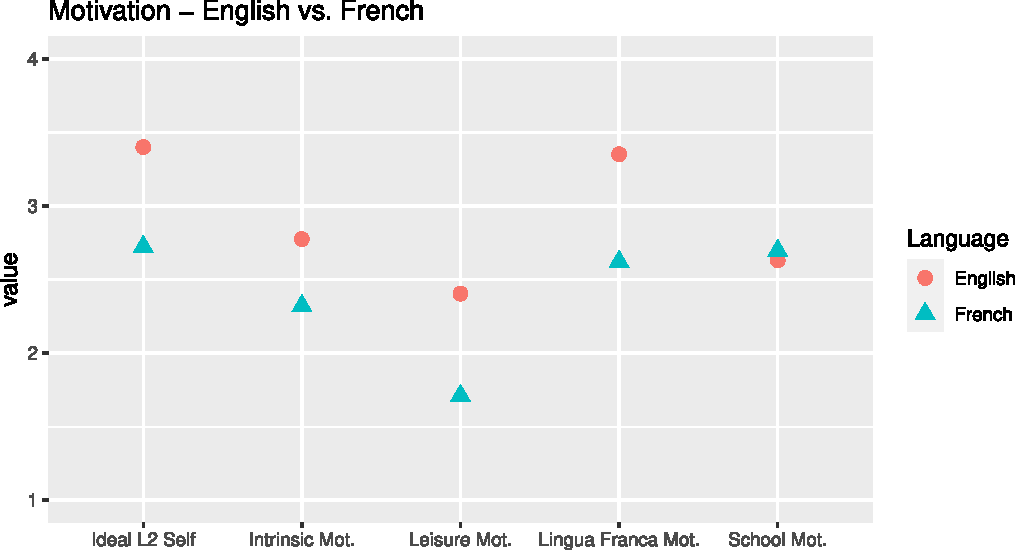
\includegraphics[width=\textwidth]{figures/Fig7.1.pdf}
\caption{L2 Motivation according to target language and subdimension based on model predictions\label{fig:07:1}}
\end{figure}

In relation to the first research question, the predicted means for English and French learning motivation in the five subdimensions are presented in \figref{fig:07:1}. Our results are mostly in line with the hypotheses outlined in \sectref{sec:07:4} and suggest that primary school students in the LAPS project are generally motivated to learn foreign languages at school, however, there are marked differences between target languages and between motivational subcomponents. As \figref{fig:07:1} indicates, the pupils seem to be particularly motivated with regard to English, were all predicted means are around or above the scale mean. The ideal L2 self and the use of English for communicative purposes turn out as the two main motivators. In return, intrinsic motivation, as well as school and leisure motivation are lower. 

With regard to French, the values are generally lower. Only school motivation is approximately at the same level as in English, all other values are substantially lower. This is how the interaction between motivational subdimension and target language can be interpreted: while school motivation is similar for both languages, the gap widens markedly in the other four dimensions.

Our results corroborate previous findings in that English learning motivation is generally higher than French learning motivation (\citealt{Stoeckli2004}, \citealt{Heinzmann2010,Heinzmann2013}, \citealt{PeyerEtAl2016}, \citealt{BruehwilerLePapeRacine2017}, \citealt{PfenningerSingleton2017}). Based on \citet{Busse2017}, this difference suggests that even young learners consciously deal with the relation of these two languages and that they assign a more valuable status to English than to French (cf. also \citealt{Ushioda2017}, \citealt{BuylHousen2014}). As one of the anonymous reviewers pointed out, a further explanation for the preference for English might lay in the (perceived) difficulty of the target language, in that German-speaking students rate English as easier to learn than French.

Irrespective of the gap between the target languages, our results encouragingly support previous studies with regard to the use of the target language as a lingua franca, which seems to be one of the students’ main aspirations for foreign language learning (cf. e.g. \citealt{SchaerBader2003}, \citealt{Stoeckli2004}). Likewise, students reported high values for the ideal L2 self, which has rarely been studied with young learners (see \citealt{Henry2009} for an exception, cf. \sectref{sec:07:3} in this Chapter and \sectref{sec:08:2}, Chapter 8). This suggests that students have vivid future self-guides and that they can imagine using English and French competently in the future. In addition, the Cronbach’s α of these scales (0.81, 0.87) indicate a consistent response behaviour. However, viewing this as an entirely positive finding would be premature, because young students have been found to overestimate themselves and \citet[38]{Doernyei2009} himself argues that learners’ future self representations are not stable at this early age.

Similarity in school-related motivation in both languages has also been found in previous studies (e.g. \citealt{Stoeckli2004}). This is not surprising, insofar as it is related to an instrumentalisation of the languages with the goal of academic success. Good educational performance proves to be important for the students in our sample, irrespective of the target language.

Furthermore, low values for leisure motivation are consistent with previous findings (cf. e.g. \citealt{SchaerBader2003}, \citealt{Stoeckli2004}, \citealt{Heinzmann2013}) and this result is not surprising. English was regarded as much more important than French, which can be linked to the greater benefits in terms of its use on the internet and in computer games. At the same time, the comparatively weaker Cronbach’s α and the fact, that even the values for English are comparatively low, suggest that such goals might not yet be highly relevant for primary school students.

A point that requires further discussion is intrinsic motivation. In accordance with other studies in similar contexts, intrinsic motivation for English is higher than for French. But in our data, intrinsic motivation for English is only slightly above the scale mean, the values for French are slightly below. Based on \citegen{DeciRyan1985ZweiterEintrag} SDT and on the repeatedly confirmed influence on language learning success, this is a rather discouraging result.

\subsection{Research question 2: The closer, the better?}\label{sec:07:5.2}

  
\begin{figure}
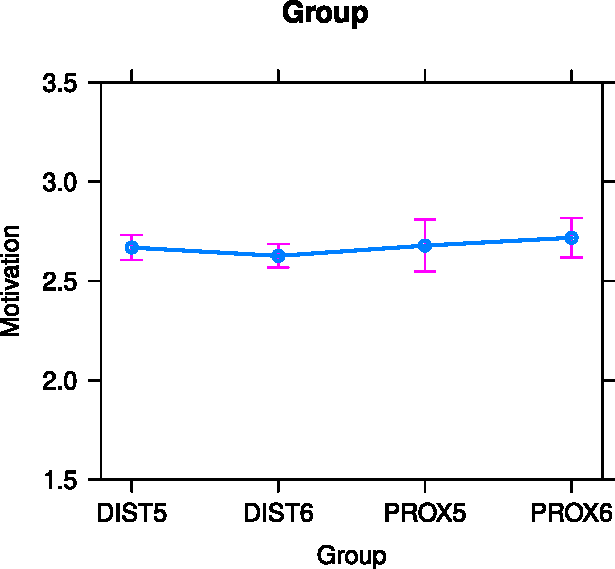
\includegraphics[width=.5\textwidth]{figures/Fig7.2.pdf}
\caption{Motivation according to learner group\label{fig:07:2}}
\end{figure}

With regard to the second research question, the model reveals no main effect for regional conditions and no interaction between regional conditions and target language. As \figref{fig:07:2} as well as the estimates displayed in \tabref{tab:07:2} suggest, all learner groups are equally motivated, irrespective of their distance to the L2 community.

According to theories that attribute a central role to the proximity to the L2 community (such as Gardner \& Lambert's socio-educational model or Clément's contact hypothesis, see Section~\ref{sec:07:2} above), an interaction between target language and student group was hypothesised: Whereas English is a ``distant'' language for both groups, they differ in geographical proximity to the French-speaking community. Thus, motivation for English would be assumed to turn out approximately the same, whereas motivation for French would be expected to be higher for children close to the French language border compared to their peers living in a region far off.

Explanations for the absence of this interaction, and thus, the absence of an effect of proximity to a speech community on the learners’ L2 motivation could be linked to the global status of the two languages being more important than the actual geographical proximity. As already mentioned above, the criticism of theories by Gardner and his associates on the relevance of a particular L2 speech community might be transferable from English to other languages (cf. also discussions in \citealt{Busse2017} and \citealt{Ushioda2017}).


\begin{figure}
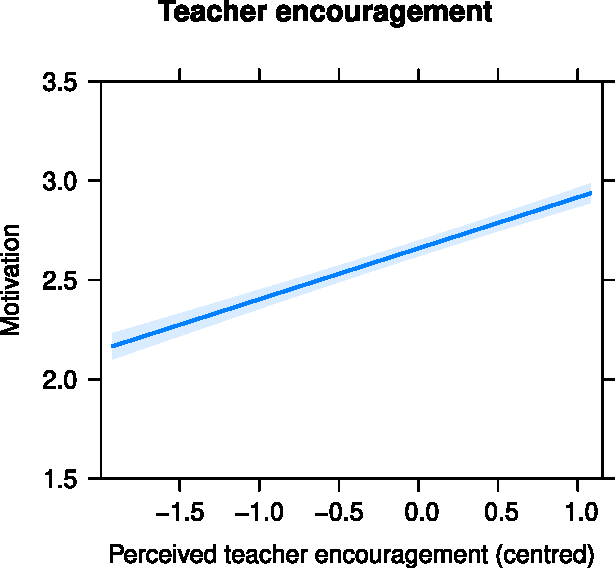
\includegraphics[width=.45\textwidth]{figures/Fig7.3.1.pdf}\hfill%
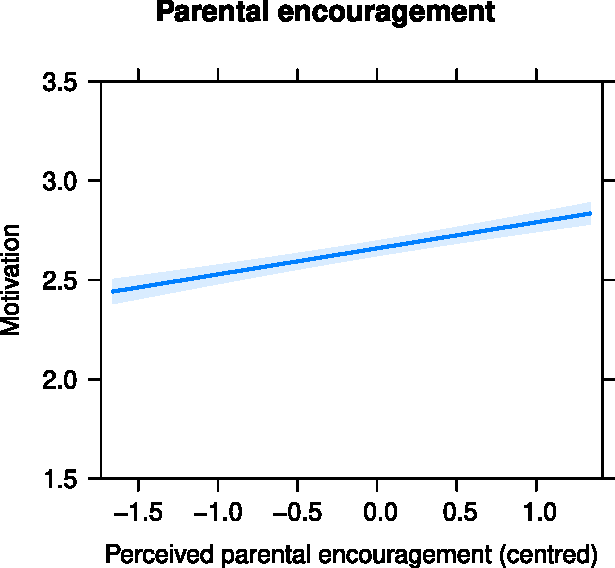
\includegraphics[width=.45\textwidth]{figures/Fig7.3.2.pdf}
\caption{Teacher and parental encouragement effect plots\label{fig:07:3}}
\end{figure}

Concerning the control variables entered in the model, perceived support by the L2 teacher seems to have a considerable impact on students’ L2 motivation (cf. \figref{fig:07:3}, left plot). To a lesser extent, this also applies to parental encouragement (cf. \figref{fig:07:3}, right plot). However, based on our data, no conclusion on the causal direction of these effects can be drawn (e.g. children who were more motivated in the first place might also perceive parental and teacher encouragement more positively).


\begin{figure}
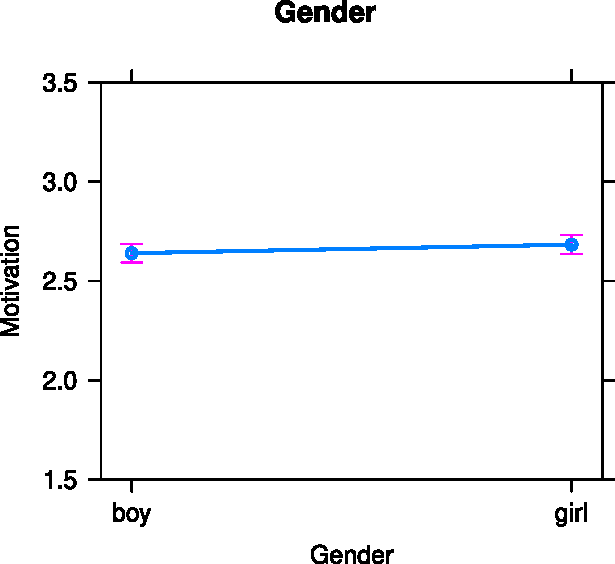
\includegraphics[width=.45\textwidth]{figures/Fig7.4.1.pdf}\hfill%
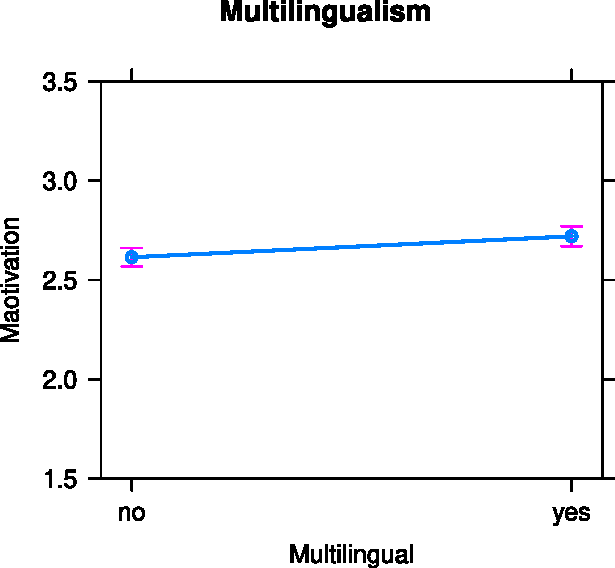
\includegraphics[width=.45\textwidth]{figures/Fig7.4.2.pdf}
\caption{Multilingualism and gender effect plots\label{fig:07:4}}
\end{figure}

In contrast, effects of multilingual background or gender were marginal (cf. \figref{fig:07:4}), and no notable between-class variation was revealed (cf. \tabref{tab:07:2}, random effect ``Class''). 

Findings from \citet{PfenningerSingleton2016} give reason to assume that the educational environment (teachers, their methodologies, peers, etc.) exerts a great influence on the individual pupils in the classroom and, thus, differences between classes should become apparent. It is therefore surprising that no evidence for substantial between-class variation was found in the current study. However, this does not imply that the teacher has no impact on his or her students. From the control variables in our model, perceived motivation and support by the teacher is the one with the greatest impact on students’ motivation. The fact that the impact of parental encouragement is comparatively lower is in line with previous findings (e.g. \citealt{Holder2005}), who showed in a qualitative approach that parental influence becomes weaker than the school environment for children at the end of primary school. 

In relation to multilingualism or gender, our data does not lend support to previous findings (\citealt{DoernyeiCsizer2002}, \citealt{Holder2005}, \citealt{Heinzmann2009,Heinzmann2010}, \citealt{BruehwilerLePapeRacine2017}, \citealt{Henry2009}, \citealt{CourtneyEtAl2017}). Whereas numerically, girls and children with a multilingual background are more motivated, these effects are modest and uncertain.

\section{Limitations}

The results of this study are subject to several limitations. Firstly, intrinsic motivation, although representing an important construct, was assessed by two items only. In order to get a more detailed view, it would be useful to gauge this construct more extensively in future studies. Secondly, the distance to the L2 community was solely based on geographical distance, direct contact with speakers of the respective community was not integrated in the questionnaire. An assessment of the intensity of interactions and contact with L2 speakers could possibly clarify the extent to which pupils actually seize opportunities to get in touch with L2 speakers and if this has an impact on their L2 motivation. Finally, the quantitative approach taken in this chapter along with a big sample (n=737) enables for generalising conclusions. At the same time, it is obvious, that such a wide-ranging construct as language learning motivation cannot be assessed comprehensively via quantitative questionnaire items alone. Additional qualitative research (e.g. via semi-structured interviews with specific learners or learner groups) could certainly provide further valuable insights.

\section{Conclusion}

With the limitations discussed above considered, a series of conclusions can be drawn from this study. In general, our data suggests that even in an educational environment, where foreign languages are part of the mandatory curriculum, pupils have various motivations for language learning beyond academic success. For instance, future self-representations and the active use of the languages for communication play a crucial role as motivators in the L2 learning process. This particularly applies to English, which is strongly favoured over French in all but the educational subdimension. The most striking result is related to the distance to an L2 community. Contrary to our expectations, the results of the current study don’t support the conclusion that proximity to the French speaking community fosters motivation to learn the respective language. As already discussed above, this might possibly be explained by the mandatory school context and the children attributing a higher status to English than to French. A closer look at the actual willingness to and intensity of contact to L2 speakers could shed more light on this intriguing finding. As to the other factors integrated in the analysis, the teacher proved to be the most important social agent in fostering pupils’ L2 motivation, whereas parents seem to exert less influence. Finally, no considerable effect of multilingualism and gender could be identified in the current study.


{\sloppy\printbibliography[heading=subbibliography,notkeyword=this]}
\end{document}
